\documentclass[14pt]{article}
\usepackage{tikz}
\usepackage{amsmath}

\begin{document}
\section*{Finance and Money Questions}
\begin{enumerate}
\item Use the loanable funds theory to explain what happens to international interest rates as China becomes a more significant world economy.  Remember that China saves a much larger proportion of its GDP than most other countries. 

\textbf{Answer}
China provides a large amount of savings to the world economy.  If this loanable funds represents the world, this will increase the supply of loanable funds (savings) from $S-1$ to $S_2$.  This will reduce the price of loanable funds (interest rate) and will increase the quantity utilised.  The demand curve already shows that there is higher demand for funds at a lower price (rate). 

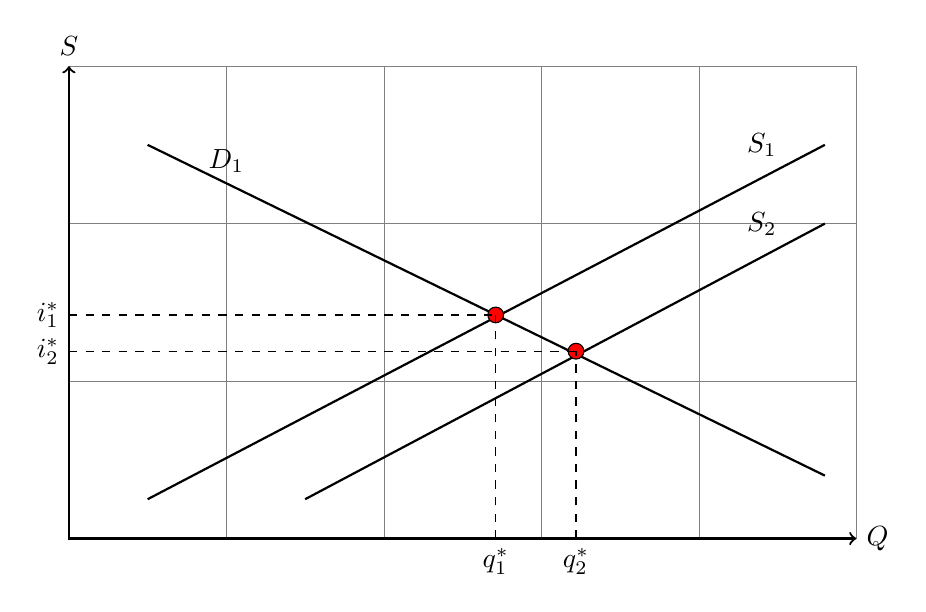
\begin{tikzpicture}[scale = 2]
\draw[very thin, color = gray](0, 0) grid (5, 3);
\draw [<->, thick] (0, 3) node (yaxis) [above] {$S$} 
  |- (5, 0) node (xaxis) [right] {$Q$};;
\draw[thick] (0.5, 2.5) to (4.8, 0.4);
\draw[thick] (0.5, 0.25) to (4.8, 2.5);
\node at (4.4, 2.5) {$S_1$};
\node at (1, 2.4) {$D_1$};
\draw [fill = red] (2.71, 1.42) circle [radius = 0.05];
\draw [dashed] (2.71, 0) to (2.71, 1.42);
\draw [dashed] (0, 1.42) to (2.71, 1.42);
\node at (2.71, 0) [below] {$q_1^*$};
\node at (0, 1.42) [left] {$i_1^*$};
\draw[thick] (1.5, 0.25) to (4.8, 2);
\node at (4.4, 2) {$S_2$};
\draw [fill = red] (3.22, 1.19) circle [radius = 0.05];
\draw [dashed] (3.22, 0) to (3.22, 1.19);
\draw [dashed] (0, 1.19) to (3.22, 1.19);
\node at (3.22, 0) [below] {$q_2^*$};
\node at (0, 1.19) [left] {$i_2^*$};

%\draw [<->, thick] (0, 3) node (yaxis) [above] {$i$} 
%  |- (5, 0) node (xaxis) [right] {$Q$};
%\node at (5, 2) [above left] {AC};
%\node at (4, 2.5) [above left] {MC};
%\draw[domain = 0.1:3.9, color = blue] plot(\x, {2 - 0.5*\x});
\end{tikzpicture}

\item How does a tax on consumption affect interest rates?

\textbf{Answer}
The picture is the same as above. The tax makes consumption more expensive and this should encourage more savings.  The savings function moves from $S_1$ to $S_2$, rates fall and the amount of loanable funds used increases. 

\item Considering two of the functions of money: means of transaction and store of value; what are the main factors affecting each of these types of demand?

\textbf{Answer}
\begin{itemize}
\item \textbf{Means of transaction}:  GDP and price level.  The more transactions and the more that they cost, the higher the transaction demand for money. 
\item \textbf{Store of value}: Level of inflation, expectations of the exchange rate, confidence.  The more the currency is expected to hold is value (inflation and exchange rate), the more it will be used as a store of value; the more that people want to save (to protect against an uncertain future), the more savings demand for money there will be. It is also possible to add the attraction of alternative savings vehicles. 
\end{itemize}

\item Use your answer to the previous question to sketch the factors that would be useful in a \emph{money-demand function}

\textbf{Answer}
\begin{equation*}
M_d = f(\underbrace{Y}_{+}, \underbrace{P}_{+} \underbrace{i}_{-}, \underbrace{C}_{-})
\end{equation*}

\item What do \emph{open-market operations} seek to achieve. 

\textbf{Answer}
These will seek to add money to the banking system. This may be to deal with temporary changes in the demand for money or to permanently change the equilibrium level of interest rates. 

\item Use a supply-and-demand diagram to show how the market for inter-bank loans would react at the weekend if the Bank of England were to refrain from taking any action. 

\textbf{Answer}
There would be an increase in the demand for money as a result of the increase in demand for money at the weekend.  With no increase in supply, the rate would increase. 

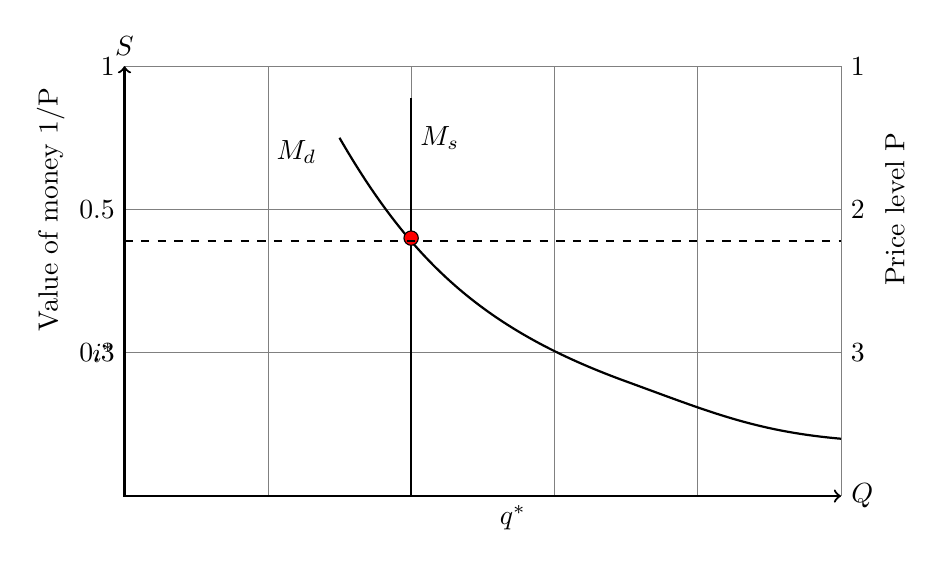
\begin{tikzpicture}[scale = 1.82]
\draw[very thin, color = gray](0, 0) grid (5, 3);
\draw [<->, thick] (0, 3) node (yaxis) [above] {$S$} 
  |- (5, 0) node (xaxis) [right] {$Q$};;
\draw[thick] (1.5, 2.5) to [out = -60, in = 160] (3.5, 0.8) to [out = -20, in = 175] (5, 0.4);
%\draw[thick] (0.5, 0.25) to [out = 0, in = 200] (3.5, 1) to [out = 20, in = 220] (5, 2);
\draw[thick] (2, 0) to (2, 2.78);
\node at (2.2, 2.5) {$M_s$};
\node at (1.2, 2.4) {$M_d$};
\draw [fill = red] (2, 1.8) circle [radius = 0.05];
\draw [dashed] (0, 1.78) to (5, 1.78);
\draw [dashed] (2, 0) to (2, 1);
\node at (2.71, 0) [below] {$q^*$};
\node at (0, 1) [left] {$i^*$};
\node at (-0.35, 2) [above, rotate = 90] {Value of money 1/P};
\node at (5.24, 2) [below, rotate = 90] {Price level P};
\node at (5, 1) [right] {3};
\node at (5, 2) [right] {2};
\node at (5, 3) [right] {1};
\node at (0, 1) [left] {0.3};
\node at (0, 2) [left] {0.5};
\node at (0, 3) [left] {1};
\end{tikzpicture}

\item Using the concept of the \emph{money multiplier} calculate the effect of a \textsterling 10 million increase in base money under the assumption that banks will lend as much as they can, that households and business are willing to borrow as much as is offered and the reserve requirement is 10\%.  How does this change if the reserve requirement is 20\%?  What does this tell you about the use of the reserve requirement to control monetary policy? 

\textbf{Answer}
The central bank will increase base money as it did at the weekend. However, in this case, there is no increase in the demand for money.  The additional base money will encourage the bank to lend and with households prepared to borrow, this will lead to an increase in loans of 
\textsterling 10 million.  Increasing loans is the same as increasing deposits.  Therefore, deposits and cash will increase by \textsterling 10 million.  However, with a reserve requirement of 10\%, \textsterling 1 million must be set aside in the reserve and the increase in available cash is just \textsterling 9 million.  This \textsterling 9 million can be lent out but will require a \textsterling 900,000 reserve requirement (10\% of \textsterling 9 million), leaving \textsterling 810,000 million to be lent.  This process continues. 

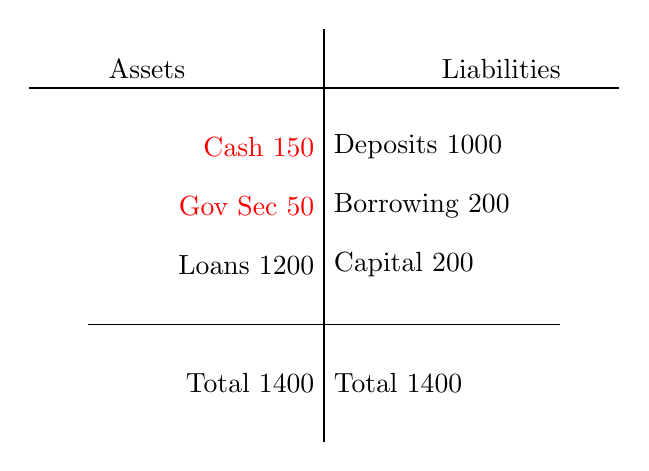
\begin{tikzpicture}[scale = 0.75]
%\draw [very thin, color = gray](0, 0) grid (14, 7);
\draw [thick] (2, 6) to (12, 6);
\draw [thick] (7, 7) to (7, 0);
\node [above] at (10, 6) {Liabilities};
\node [above] at (4, 6) {Assets};
\node [right] at (7, 5) {Deposits 1000};
\node [left, color = red] at (7, 5) {Cash 150};
\node [right] at (7, 4) {Borrowing 200};
\node [left, color = red] at (7, 4) {Gov Sec 50};
\draw (3, 2) to (11, 2);
\node [right] at (7, 3) {Capital 200};
\node [left] at (7, 3) {Loans 1200};
\node [right] at (7, 1) {Total 1400};
\node [left] at (7, 1) {Total 1400};
\end{tikzpicture}


With a larger reserve requirement, there is more leakage out of the process and the effect of the \emph{money multiplier} is less powerful. This can be quantified. 

If 10m is the increase in base money, RR is the reserve requirement, the total increase in broad money is $\Delta M$, then

\begin{equation}\label{eqref1}
\Delta M = 10m + (1-RR) \times 10m + (1-RR)^2 \times 10m + (1-RR)^3 \times 10m \dots + (1-RR)^{\infty} \times 10m
\end{equation}

Multiply each side by $(1+RR)$ will give

\begin{equation}\label{eqref2}
\Delta M \times (1+RR) = 10m \times (1+RR) + (1-RR)^2 10m + (1-RR)^3 \times 10m + \dots + (1-RR)^{\infty} \times 10m
\end{equation}

Now take Equation \ref{eqref2} from Equation \ref{eqref1}

\begin{equation}\label{eqref3}
\Delta M - \Delta M \times (1+RR) = 10m + \dots (1-RR)^{\infty} \times 10m
\end{equation}

However, as $(1-RR)^{\infty}$ is very close to zero, we have 

\begin{equation}
\Delta M - \Delta M \times (1+RR) = 10m
\end{equation} 

Therefore, 

\begin{equation}
\Delta M \left [1 - (1-RR) \right] = 10m
\end{equation}

Therefore, 

\begin{equation}
\Delta M = \frac{10m}{1 - (1-RR)}  
\end{equation}

As the RR is 10\%, 

\begin{equation*}
\Delta M = \frac{10m}{0.1} = 100m
\end{equation*}

Therefore, if the reserve requirement is 20\%, 

\begin{equation*}
\Delta M = \frac{10m}{0.2} = 50m
\end{equation*}

The reserve requirement reduces the power of the money multiplier.

\end{enumerate}


\end{document}
